\section{Material Optimization}

\begin{frame}{1D Example}
\begin{figure}
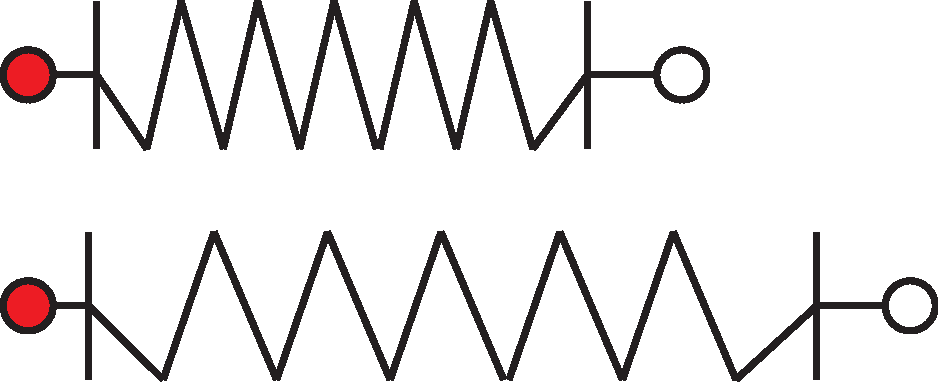
\includegraphics[width=0.6\textwidth]{Images/spring_stretch.pdf}
\end{figure}

\begin{itemize}
\item Hook's law: $F = -k u$
\pause \item In 1D, Force $F$ and displacement $u$ are coupled through spring constant $k$.
\pause \item In 3D, stress $\sigma$ and strain $\epsilon$ are coupled through
material tensor.
\end{itemize}
\end{frame}

\begin{frame}{Discretize material properties}
\begin{figure}
\hspace{\fill}
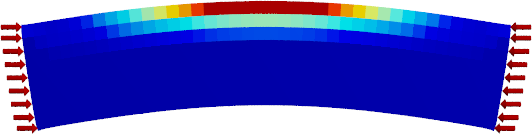
\includegraphics[width=0.45\textwidth]{Images/material_opt_half_period.png}
\hspace{\fill}
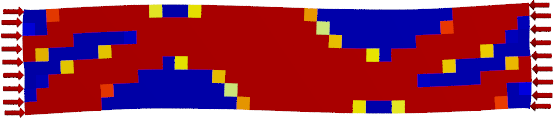
\includegraphics[width=0.45\textwidth]{Images/material_opt_full_period.png}
\hspace{\fill}

\vspace{3mm}
\hspace{\fill}
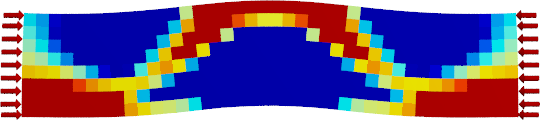
\includegraphics[width=0.45\textwidth]{Images/material_opt_bump_half.png}
\hspace{\fill}
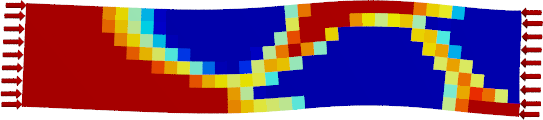
\includegraphics[width=0.45\textwidth]{Images/material_opt_bump_third.png}
\hspace{\fill}
\end{figure}

\begin{itemize}
\item Homogeneous material properties is very restrictive.
Heterogeneous material is needed to achieve interesting examples.
\end{itemize}
\end{frame}

\begin{frame}{Material optimization}
\begin{align*}
\min_{E, \nu} & \int_{\partial \Omega} \|u - u^*\|^2 \dA\\
\textrm{s.t.} & \nabla \cdot \sigma(u) = f \qquad \forall x \in \Omega\\
& \sigma(u) \cdot n = t \qquad \forall x \in \partial \Omega_{N}
\end{align*}
where $E,\nu : \Omega \to \mathbb{R}$.

\begin{itemize}
\pause \item The optimal solution is not unique.
\pause \item The constraint is a PDE.
\end{itemize}
\end{frame}

\begin{frame}{What we have tried?}
\begin{itemize}
\item Gradient-based algorithm: gradient descent, BFGS.
\item A local/global iteration algorithm.
\begin{itemize}
\item Compute strain with only Dirichlet BC enforced.
\item Compute stress with only Neumann BC enforced.
\item Fit material properties using constrained nonlinear least sqaure.
\end{itemize}
\end{itemize}
\end{frame}

\begin{frame}{Results}
\begin{figure}
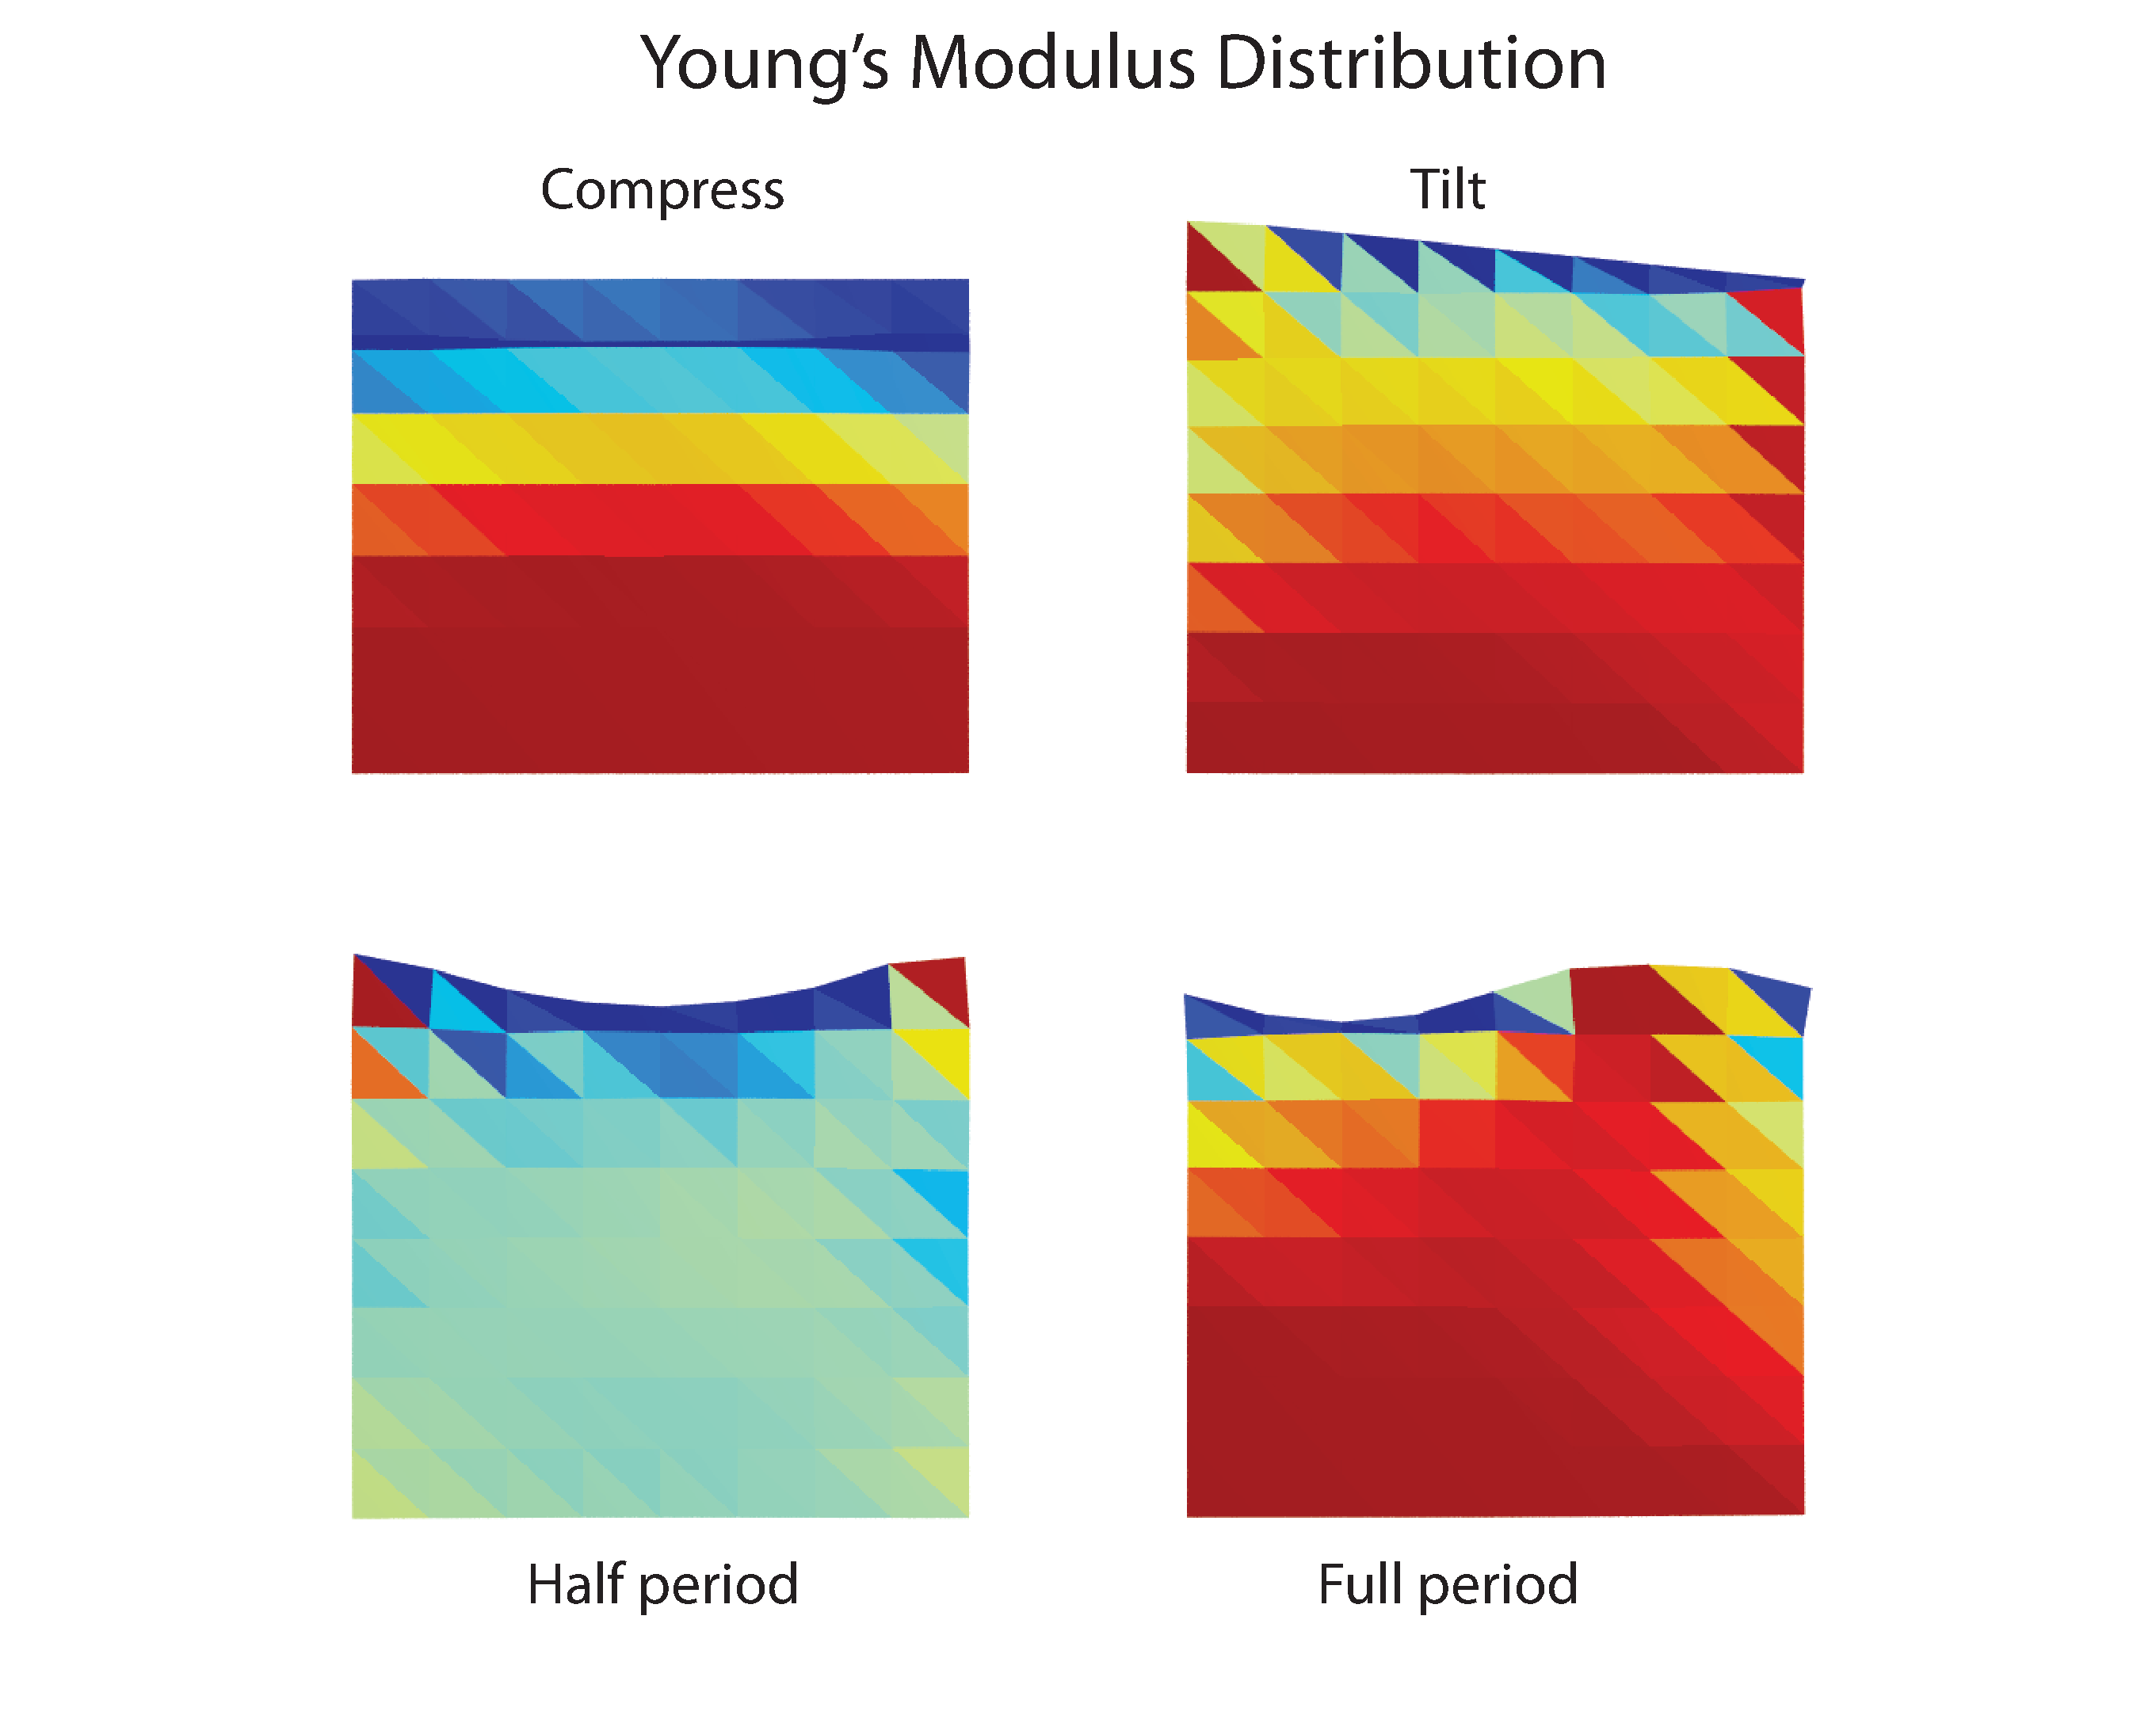
\includegraphics[width=0.9\textwidth]{Images/box_compression_test.pdf}
\end{figure}

\end{frame}


